\let\negmedspace\undefined
\let\negthickspace\undefined
\documentclass[journal]{IEEEtran}
\usepackage[a5paper, margin=10mm, onecolumn]{geometry}
%\usepackage{lmodern} % Ensure lmodern is loaded for pdflatex
\usepackage{tfrupee} % Include tfrupee package

\setlength{\headheight}{1cm} % Set the height of the header box
\setlength{\headsep}{0mm}     % Set the distance between the header box and the top of the text

\usepackage{gvv-book}
\usepackage{gvv}
\usepackage{cite}
\usepackage{amsmath,amssymb,amsfonts,amsthm}
\usepackage{algorithmic}
\usepackage{graphicx}
\usepackage{textcomp}
\usepackage{xcolor}
\usepackage{txfonts}
\usepackage{listings}
\usepackage{enumitem}
\usepackage{mathtools}
\usepackage{gensymb}
\usepackage{comment}
\usepackage[breaklinks=true]{hyperref}
\usepackage{tkz-euclide} 
\usepackage{tikz}
\usepackage{listings}
\usetikzlibrary{patterns}
% \usepackage{gvv}                                        
\def\inputGnumericTable{}                                 
\usepackage[latin1]{inputenc}                                
\usepackage{color}                                            
\usepackage{array}                                            
\usepackage{longtable}                                       
\usepackage{calc}                                             
\usepackage{multirow}                                         
\usepackage{hhline}                                           
\usepackage{ifthen}                                           
\usepackage{lscape}
\begin{document}
\bibliographystyle{IEEEtran}
\vspace{3cm}

\title{GATE\\AE - 2011}
\author{EE24BTECH11061 - Rohith Sai}
\maketitle

\renewcommand{\thefigure}{\theenumi}
\renewcommand{\thetable}{\theenumi}

\section*{Multiple Choice Type}
\begin{enumerate}
\item An aircraft with a mass of 5000 kg takes off from sea level with a forward speed of 50 m/s and starts to climb with a climb angle of $15 \degree$. The rate of climb and excess thrust available at the start of the climb respectively $\brak{\text{assume }g = 9.81 ms^{-2}}$ are
\begin{multicols}{2}
    \begin{enumerate}
        \item 13.40 m/s and 13146.0 N
        \item 12.94 m/s and 12694.1 N
        \item 13.40 m/s and 12694.1 N
        \item 12.94 m/s and 13146.0 N
    \end{enumerate}
\end{multicols}

\item A glider having a mass of 500 kg is taken to an altitude of 1000 m with a jeep moving on ground at 54 kmph. Upon reaching the required altitude in 50 s, the glider is released and starts its descent. Under the assumption of equilibrium glide, the range and endurance of the glider for a constant lift-to-drag ratio of 15 are
\begin{multicols}{2}
    \begin{enumerate}
        \item 15.0 km and 1002.2 s respectively
        \item 15.0 km and 601.3 s respectively
        \item 1.0 km and 601.3 s respectively
        \item 1.0 km and 50 s respectively
    \end{enumerate}
\end{multicols}
    
\item An elliptic orbit has its perigee at 400 km above the Earth's surface and apogee at 3400 km above the Earth's surface. For this orbit, the eccentricity and semi-major axis respectively are (assume radius of Earth = 6400 km)
\begin{multicols}{2}
    \begin{enumerate}
        \item 0.18 and 8300 km
        \item 0.18 and 1900 km
        \item 0.22 and 8300 km
        \item 0.22 and 1900 km
    \end{enumerate}
\end{multicols}

\item An aircraft in level flight encounters a vertical gust, which excites the phugoid mode. The phugoid motion completes 10 cycles in 50 s and its amplitude reduces to half of its maximum value in 25 s. The eigenvalues of the phugoid mode are
\begin{multicols}{2}
    \begin{enumerate}
        \item $-0.05 \pm 0.02 \iota$
        \item $-0.5 \pm 0.2 \iota$
        \item $-0.028 \pm 1.26 \iota$
        \item $0.028 \pm 1.26 \iota$
    \end{enumerate}
\end{multicols}

\item Consider the inviscid, adiabatic flow of air at free stream conditions, $M_1 = 2$, $p_1 = 1$ atm and $T_1 = 288$ K around a sharp expansion corner $\brak{\theta = 20 \degree}$ as shown below. The Prandtl-Meyer function, $v$, is given as a function of Mach number, $M$, as $v(M) = \sqrt{\frac{\gamma + 1}{\gamma - 1}} \tan^{-1} \sqrt{\frac{\gamma - 1}{\gamma + 1}\brak{M^2 - 1}} - \tan^{-1} \sqrt{M^2 - 1}$
Assume air to be calorically perfect with $\gamma = 1.4$. The Mach number, $M_2$, downstream of the expansion corner is approximately
\begin{tikzpicture}

    % Draw the horizontal surface
    \draw[thick] (-4,0) -- (0,0);
    
    % Draw the inclined surface
    \draw[thick] (0,0) -- (3,-1);
    
    % Draw dashed horizontal extension
    \draw[dashed] (0,0) -- (3,0);
    
    % Add hashed shading below the horizontal line
    \fill[pattern=north east lines, pattern color=black] (-4,-0.3) rectangle (0,0);

    % Add hashed shading below the inclined line with thickness 0.3
    \fill[pattern=north east lines, pattern color=black] (0,-0.3) -- ++(3,-1) -- ++(0,0.3) -- ++(-3,1) -- cycle;

    % Add arrows representing flow direction
    \draw[->, thick, gray] (-3.5,0.5) -- (-1.5,0.5); % M1 arrow along horizontal

    % M2 arrow above incline at a parallel distance of 0.5
    \draw[->, thick, gray] (1.5, -0.25) -- ++(1.5,-0.5); % Adjust starting position to be above the incline

    % Label flow parameters
    \node[anchor=south] at (-2.5,0.5) {$M_1, p_1, T_1$};
    \node[anchor=south] at (2.5,-0.5) {$M_2$}; % Adjust label position for M2

    % Draw the angle arc
    \draw[thick] (1,0) arc[start angle=0, end angle=-18, radius=1] node[midway, right] {$\theta$};

\end{tikzpicture}
\begin{multicols}{2}
    \begin{enumerate}
        \item 2.48
        \item 2.31
        \item 2.60
        \item 2.89
    \end{enumerate}
\end{multicols}

\item Consider a steady two dimensional zero-pressure gradient laminar flow of air over a flat plate as shown below. The free stream conditions are $U_{\infty} = 100$ ms$^{-1}$, $\rho_{\infty} = 1.2$ kg m$^{-3}$, $p_{\infty} = 1$ atm and $\mu_{\infty} = 1.8 \times 10^{-5}$ kg m $^{-1}$ s $^{-1}$. The ratio of displacement thickness to momentum thickness of the boundary layer at a distance of 2 m from the leading edge is
\begin{tikzpicture}
    % Define the coordinates
    \draw[thick] (0,0) -- (6,0);  % Plate
    \draw[thick] (0,0) -- (0,-0.5);  % Vertical line at the start of the plate
    \draw[thick] (4,-0.5) -- (4,0); % Small line at 2m
    
    % Boundary layer curve
    \draw[thick] plot [smooth] coordinates {(0,0) (0.1,0.05) (1.5,0.25) (2,0.3) (3,0.4) (4,0.45) (5,0.5) (6,0.55)};

    \fill[pattern=north east lines, pattern color=black] (0,0) rectangle (6,-0.2);
    
    % Flow arrow
    \draw[->, thick] (-2,0.25) -- (0,0.25);
    \node at (-2.5,0.25) {${\mu_\infty}$};
    
    % Boundary layer label
    \draw[->] (5,0.8) -- (4.7,0.5);
    \node at (5,0.9) {Boundary layer};
    
    % 2m label
    \draw[<->] (0,-0.3) -- (4,-0.3);
    \node at (2,-0.5) {2 m};
    
    % Symbols on the left side
    \node at (-2.5,0.5) {$p_\infty$};
    \node at (-2.5,0.75) {$\rho_\infty$};
    \node at (-2.5,1) {$U_\infty$};
    
\end{tikzpicture}
\begin{multicols}{2}
    \begin{enumerate}
        \item 7.53
        \item 2.59
        \item 2.91
        \item 0.39
    \end{enumerate}
\end{multicols}

\item In the context of Prandtl's lifting line theory for a finite wing, which of the following combinations of statements is \textbf{TRUE}?
P: The bound vertex is responsible for the lift force
Q: The trailing vortices are responsible for the induced drag
R: The bound vortex is responsible for the induced drag
S: The trailing vortices are responsible for the lift force
\begin{multicols}{2}
    \begin{enumerate}
        \item P,Q  
        \item Q,R
        \item R,S
        \item P,S
    \end{enumerate}
\end{multicols}

\item Consider flow over a thin aerofoil at Mach number, $M_{\infty} = 0.5$ at an angle of attack, $\alpha$. Using the Prandtl-Glauert rule for compressibility correction, the formula for lift coefficient, $c_l$, can be written as
\begin{multicols}{2}
    \begin{enumerate}
        \item $5.44 \alpha$
        \item $6.28\alpha$
        \item $7.26\alpha$
        \item $14.52 \alpha$
    \end{enumerate}
\end{multicols}

\section*{Common Data Questions}
\subsection*{Common Date for Questions 48 \& 49:}
The partial differential equation (PDE) governing free vibrations of a uniform Euler-Bernoulli beam is given by $EI \frac{\partial^4 w}{\partial x^4} + m \frac{\partial^2 w}{\partial t^2} = 0$, where $EI$ is the flexural stiffness, $m$ is the mass per unit length, $w\brak{x,t}$ is the bending displacement, $x$ is the coordinate along the beam length, $t$ is time and $L$ is the beam length
\begin{tikzpicture}
    % Left boundary wall with hatching
    \fill[pattern=north east lines] (-0.3, -0.5) rectangle (0, 0.5);
    \draw[thick] (0, -0.5) -- (0, 0.5);

    % Long horizontal rectangle (channel)
    \draw[thick] (0, 0.1) -- (6, 0.1);
    \draw[thick] (0, -0.1) -- (6, -0.1);
    \draw[thick] (6, -0.1) -- (6, 0.1);

    % Flow arrows inside the channel
    \draw[->] (0, 0) -- (3, 0); % Main flow arrow from left to right

    % Labels for x = 0, x, and x = L
    \node at (0.45, 0.3) {$x = 0$};
    \node at (3, 0.3) {$x$};
    \node at (6, 0.3) {$x = L$};

    % Distance L arrow
    \draw[<->] (0, -0.4) -- (6, -0.4);
    \node at (3, -0.7) {$L$};
\end{tikzpicture}

\item To solve the PDE, the number of boundary conditions (BC) and initial conditions (IC) needed are
\begin{multicols}{2}
    \begin{enumerate}
        \item 4 BC, 3 IC
        \item 2 BC, 2 IC
        \item 2 BC, 4 IC
        \item 4 BC, 2 IC
    \end{enumerate}
\end{multicols}
\item For the cantilever beam shown in the figure, which of the following \textbf{CANNOT} be a possible boundary condition?
\begin{multicols}{2}
    \begin{enumerate}
        \item $w\brak{0,t} = 0$
        \item $\frac{\partial^2 w}{\partial x^2} \brak{L,t} = 0$
        \item $\frac{\partial^2 w}{\partial x^2} \brak{0,t} = 0$
        \item $\frac{\partial^3 w}{\partial x^3} \brak{L,t} = 0$
    \end{enumerate}
\end{multicols}

\subsection*{Common Data for Questions 50 \& 51:}
Consider an inviscid, adiabatic flow of air at free stream Mach Number, $M_{\infty} = 2$, across a compression corner $\brak{\theta = 20 \degree}$ as shown. The free stream total enthalpy is $h_{0 \infty} = 810$ kJ kg $^{-1}$. Assume that air is calorically perfect with $\gamma = 1.4$, R = 287 Jkg$^{-1}$K$^{-1}$\\
\begin{tikzpicture}
    % Ground line with hatch pattern
    \fill[pattern=north east lines] (-1,-0.1) rectangle (2,0);
    \draw[thick] (-1,0) -- (2,0); % Main ground line
    \draw[dashed] (2,0) -- (4,0);
    
    % Slanted line representing the inclined surface
    \draw[thick] (2,0) -- ++(30:2.5) coordinate (P);
    \draw[thick] (2,0) --++(60:2.25) ;
    % Point P
    \filldraw (P) circle (2pt) node[above right] {P};

    % Angle beta
    \draw[thick, ->] (2,0) ++(0:0.8) arc (0:60:0.8);
    \node at (2.8,0.7) {$\beta$};
    
    % Angle theta
    \draw[thick, ->] (2.5,0) ++(0:0.8) arc (0:30:1.3);
    \node at (3.5,0.2) {$\theta$};

    % Flow arrow for M_infinity
    \draw[->, thick] (-1,0.5) -- (1,0.5);
    \node at (-1.3,0.5) {$M_\infty$};

    % Dashed horizontal line for height measurement
    \draw[<->, thick] (P) -- (4.19,0);
    \node at (4.6,0.5) {1 m};

\end{tikzpicture}
\item The shock angle $\beta$ is
\begin{multicols}{2}
    \begin{enumerate}
        \item $=20 \degree$
        \item $>20 \degree \text{ and } <30 \degree$
        \item $ = 30 \degree$
        \item $>30 \degree$
    \end{enumerate}
\end{multicols}
\item The total temperature at point P is
\begin{multicols}{2}
    \begin{enumerate}
        \item 806.37 K
        \item 1128.92 K
        \item 1612.74 K
        \item 2257.84 K
    \end{enumerate}
\end{multicols}

\section*{Linked Answer Questions}
\subsection*{Statement for Linked Answer Questions 52 \& 53:}
A thin-walled (thickness << radius), hollow shaft of length 1m and mean radius, $R = 5$ cm has to be designed such that it can transmit a torque, $T = 7$ kN-m. A survey of different commercially available materials was made and following data was obtained from the suppliers (E : Young's Modulus, $\tau_y$ : yield stress in shear, $\rho$ : density):
\begin{tabular}[12pt]{ |c| c|}
    \hline
    \textbf{Variable} & \textbf{Description}\\ 
    \hline
    $x\brak{0}$ & First term of the AP \\
    \hline 
    $d$ & Common difference of the AP\\
    \hline
    $y\brak{n}$ & Sum of $n+1$ terms of the AP\\
    \hline
    $x\brak{n}$ & General term\\
    \hline   
    \end{tabular}[h!]
\item Which of the above materials would you choose such that weight of the shaft is minimum?
\begin{multicols}{2}
    \begin{enumerate}
        \item X only
        \item Y only
        \item Z only
        \item X or Y
    \end{enumerate}
\end{multicols}
\item If you assume a factor of safety of 2, what should be the approximate thickness of such a shaft?
\begin{multicols}{2}
    \begin{enumerate}
        \item 0.5 mm
        \item 1 mm
        \item 2 mm
        \item 4 mm
    \end{enumerate}
\end{multicols}
\end{enumerate}
\end{document}